\documentclass[12pt, a4paper]{article}
\usepackage[margin=3cm]{geometry}
\usepackage{hyperref}
\usepackage[italian]{babel}
\usepackage{background}
\usepackage{graphicx}

\hypersetup{
    colorlinks=true,
    linkcolor=orange,
    filecolor=orange,
    urlcolor=orange,
    pdftitle={Annuncio ufficiale Lancio Razzi},
    pdfauthor={Tommaso Bocchietti}
    }

\urlstyle{same}

\graphicspath{{./img/}{./pdf/}}

\backgroundsetup{
    scale=1,
    opacity=0.01,
    angle=0,
    contents={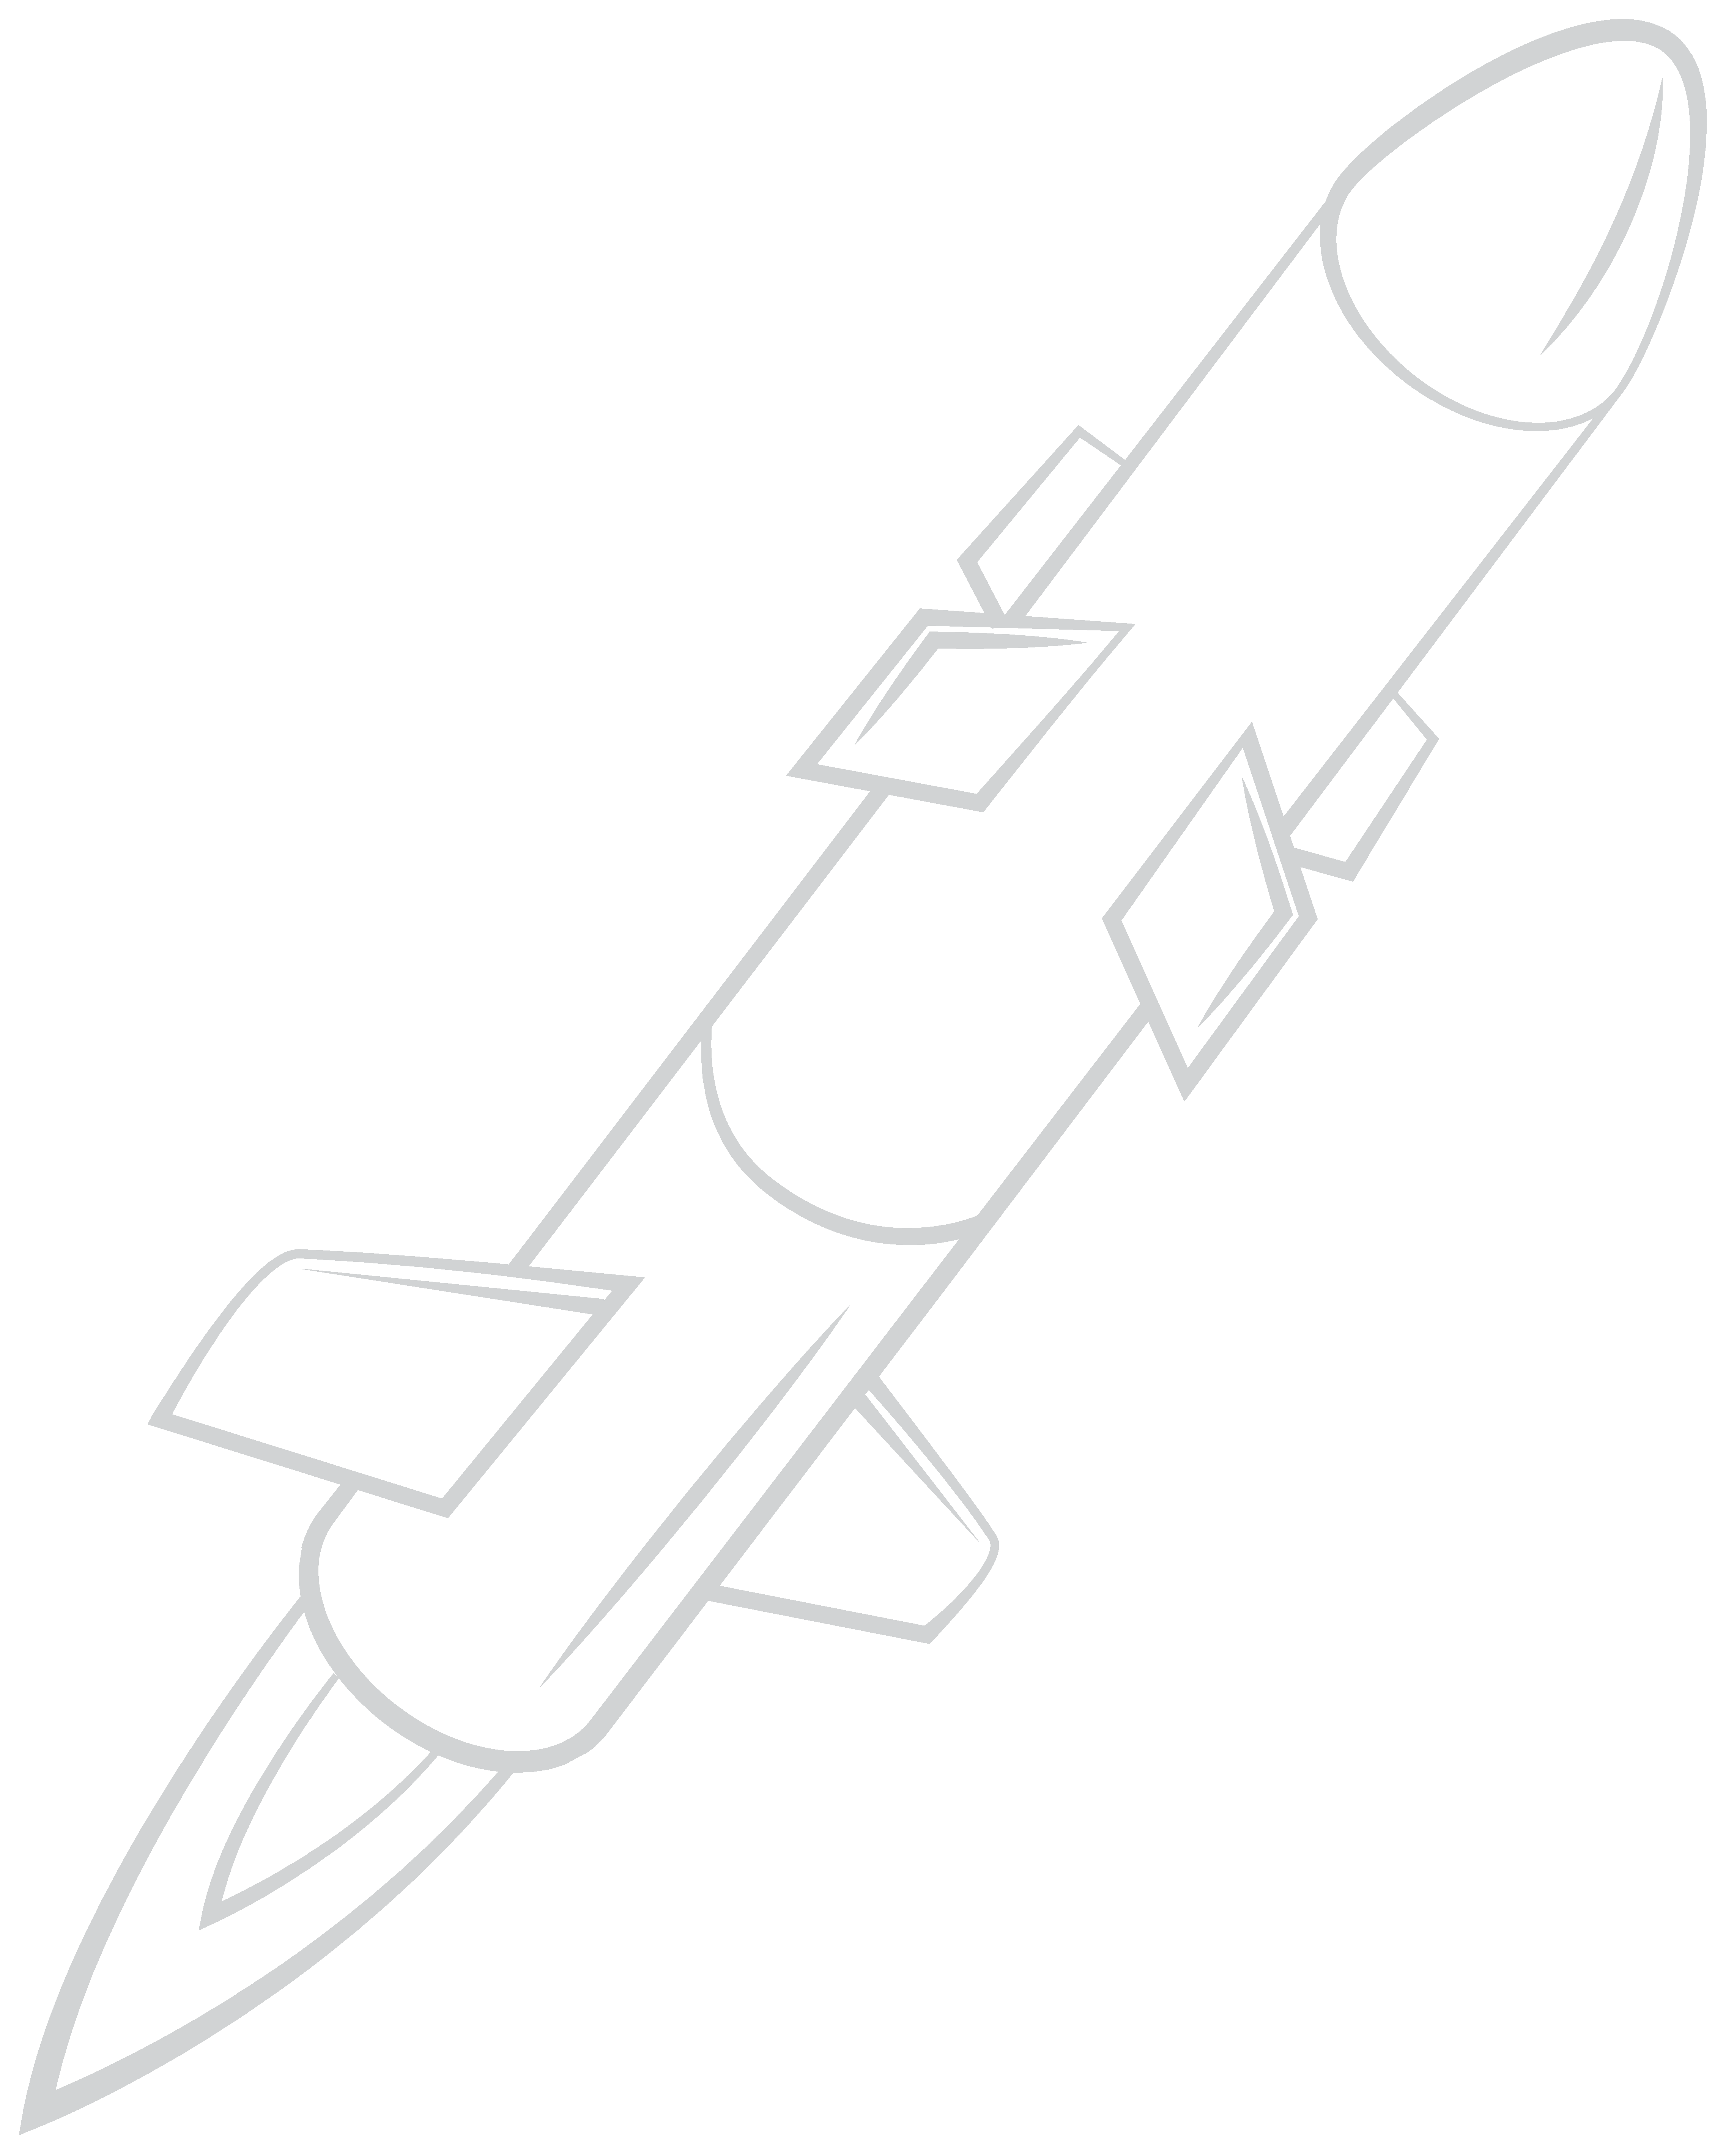
\includegraphics[width=0.6\paperwidth]{Rocket background.pdf}}
}

\begin{document}

\parbox{.35\linewidth}
{
    \begin{flushleft}
        
\includegraphics[width=2cm]{Gear bulb icon.png}\\
        % 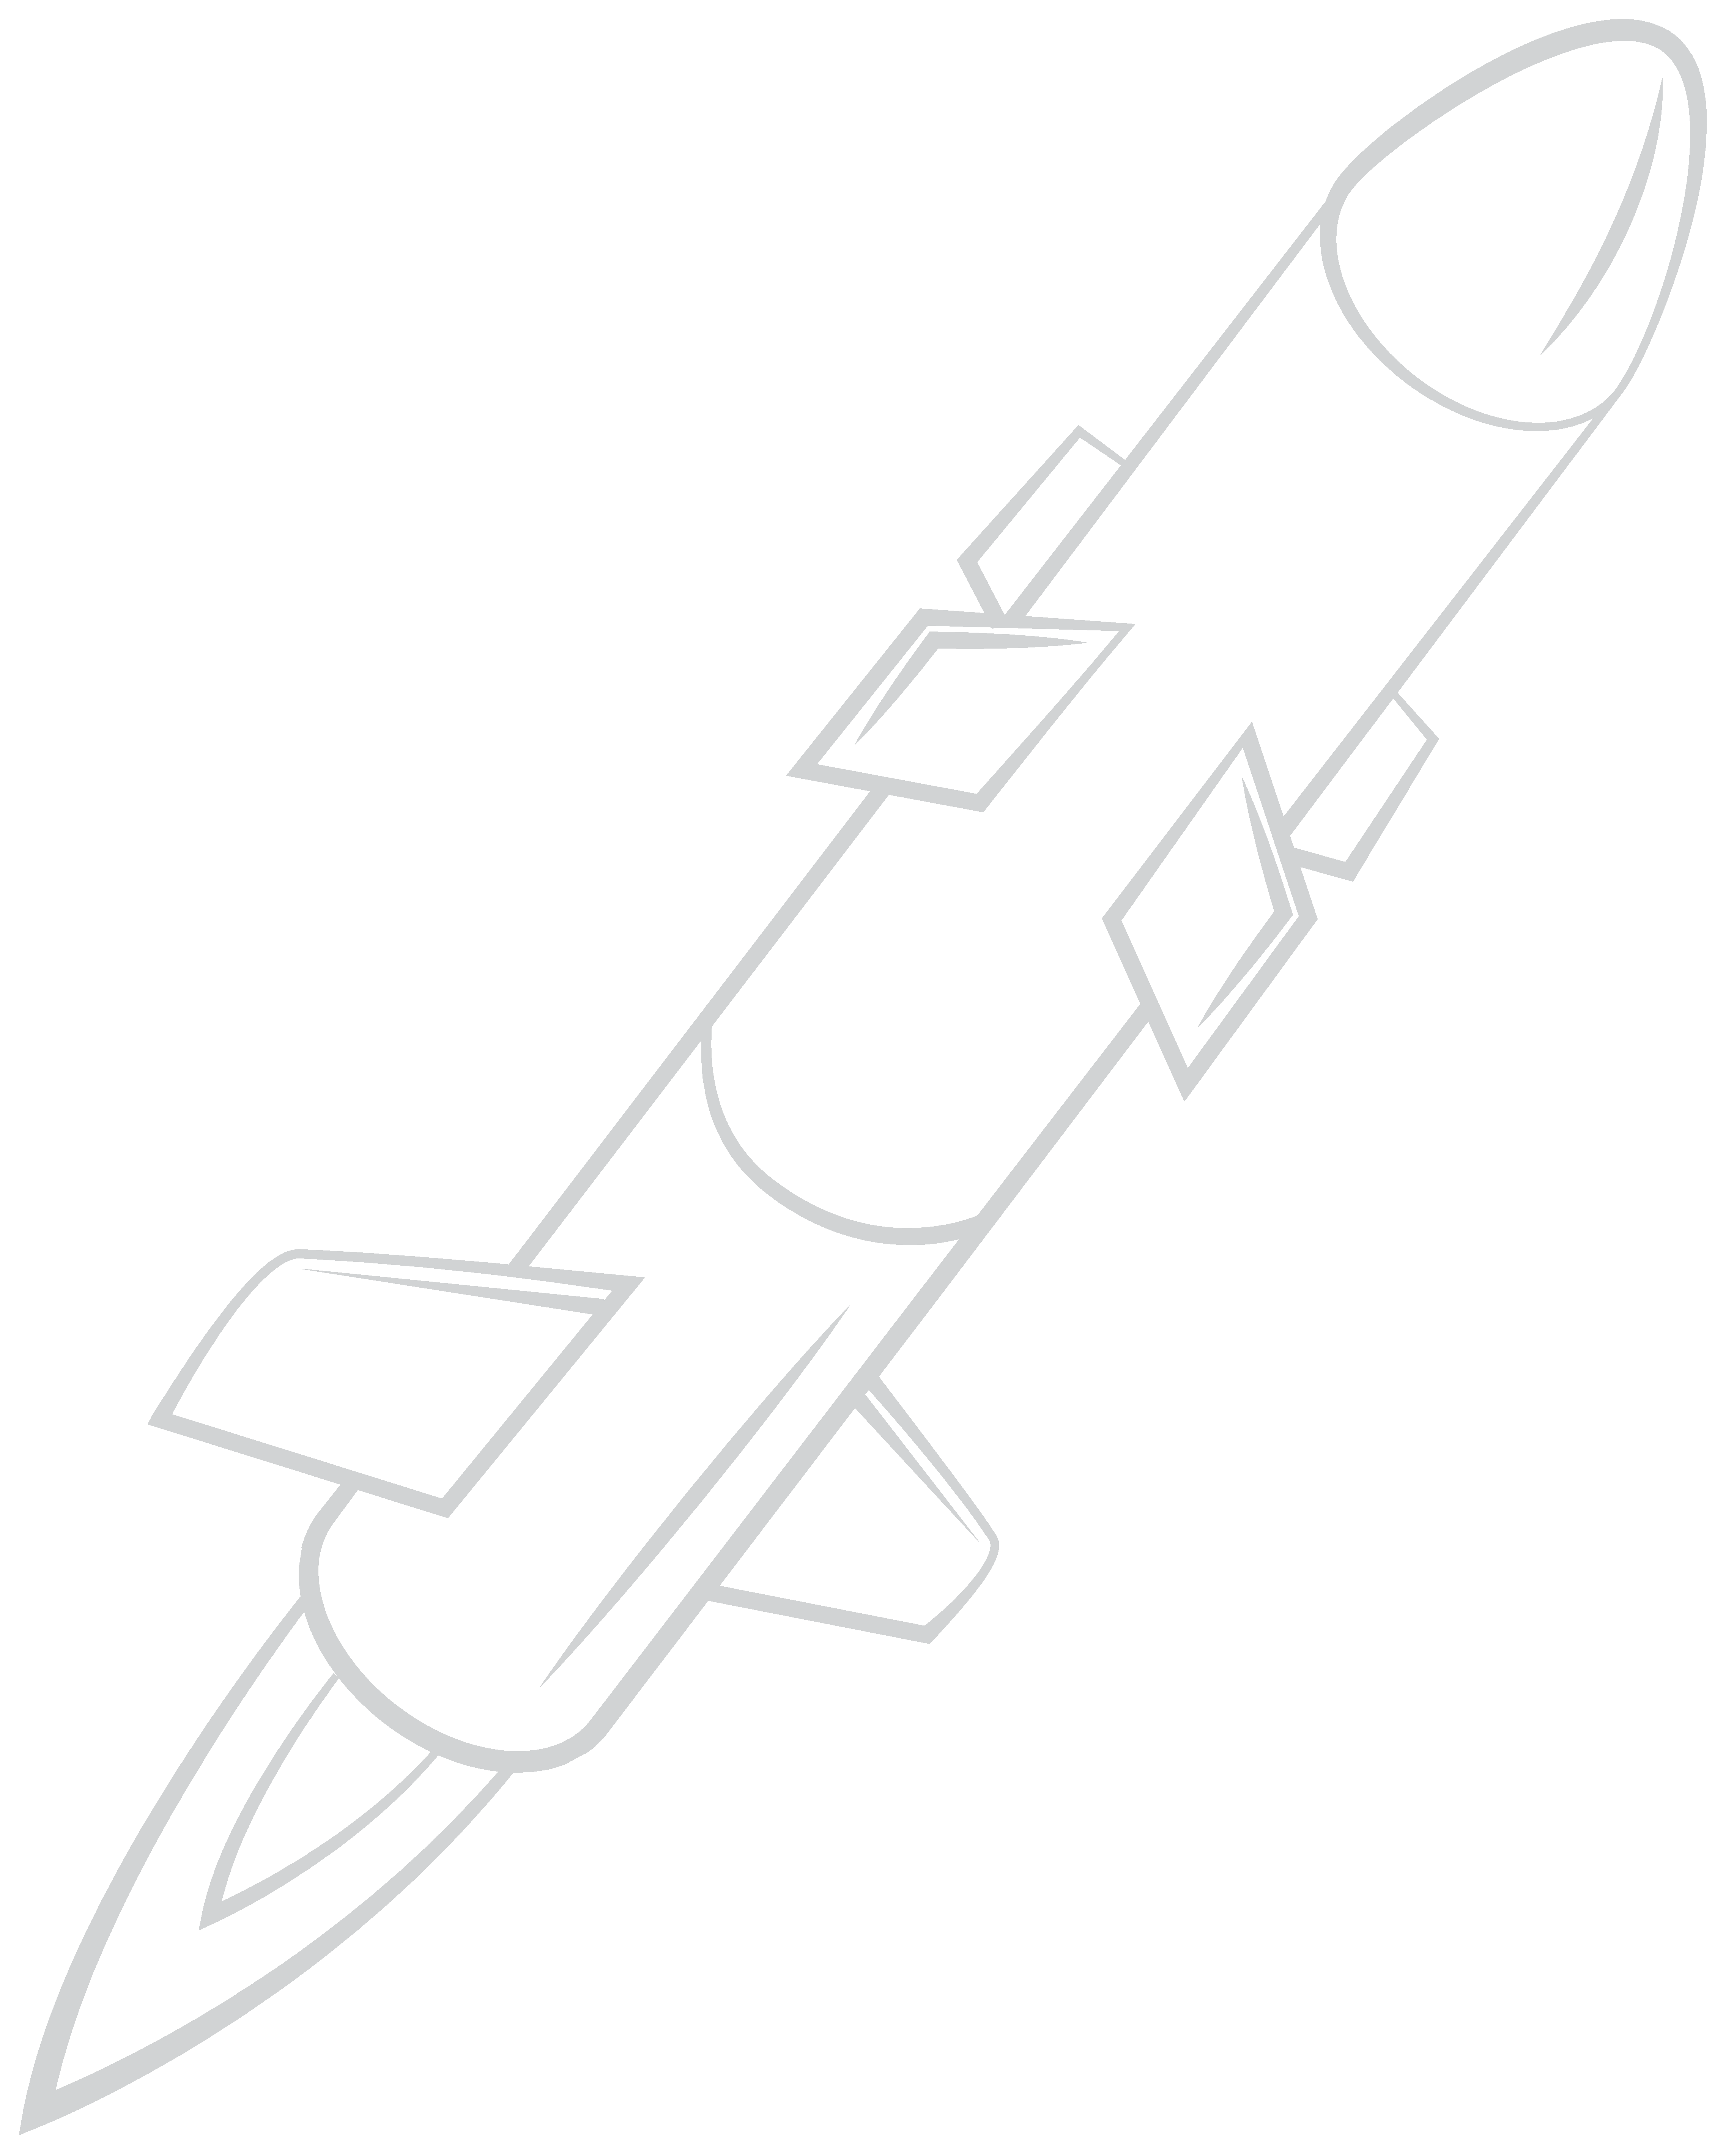
\includegraphics[width=2cm]{Rocket background.pdf}\\
    \end{flushleft}
}
\parbox{.6\linewidth}
{
    \begin{flushright}
        Laboratorio di Bocchio \\
        Sezione Aeronautica e Spazio profondo \\
        \vspace{1em}
        \today \\
    \end{flushright}
}

\vspace{3em}

\noindent Compagni di avventura \\
Amici di vario legame \\
Chiunque altro abbia voglia di vedere due missili partire verso l'ignoto \\

% Letter style
\setlength{\parindent}{0pt}
\setlength{\parskip}{1.5em}

È con grande entusiasmo ed emozione che il sottoscritto \textbf{Bocchio è lieto di annunciare il primo lancio dei suoi razzi fatti in casa!}

Come alcuni di voi già sanno, il \dateitalian{21/07/2023} Bocchio si laureerà in Ingegneria Meccanica e per festeggiare ha deciso di condividere con tutti voi questo suo nuovo progetto (ennesimo direbbe qualcuno...).

\textbf{Questa lettera vuole quindi essere un invito ufficiale a partecipare a questo evento speciale} che si terrà sulla \href{https://goo.gl/maps/K2kVRpBknDxLTATeA}{cima del Monte Crocione a San Fedele Intelvi} nel pomeriggio/sera della stessa data.
Maggiori dettagli saranno forniti nelle pagine seguenti.

Colgo l'occasione per ringraziare tutti coloro che hanno (per lo più inconsciamente) contribuito alla realizzazione di questo progetto.

\vspace{3em}

Augurandomi di potervi vedere tutti belli carichi e muniti di scudi protettivi per eventuali razzi birichini e vaganti, Bocchio vi saluta e vi aspetta.


\clearpage
\newpage
\setlength{\parindent}{1em}
\setlength{\parskip}{1pt}


\section{Scopo dell'evento}

Ufficialmente, lo scopo dell'evento è quello di festeggiare la laurea di Bocchio. \\
In realtà, se stai leggendo questa lettera significa che per un motivo o per l'altro ho interesse a condividere con te questo momento.
Volendo entrare nello specifico, tra le possibili ragioni del perchè tu sia stato/a invitato/a ci sono:
\begin{itemize}
    \item Sei un amico stretto di Bocchio
    \item Ci conosciamo da poco ma ti sei dimostrato/a una persona interessante e mi piacerebbe aprirmi con te mostrandomi questa parte più creativa di me
    \item Ci conosciamo abbastanza bene e penso che tu possa trarre ispirazione da questo evento/progetto per il tuo futuro
    \item É da tanto che non ci vediamo, mi piacerebbe rivederti e ho pensato potesse essere interessante per entrambi trovarsi per una attività diversa dal solito
\end{itemize}


\section{Programma di massima}

Il programma dell'evento è stato organizzato in modo da offrire un'esperienza coinvolgente, divertente e accessibile per tutti i partecipanti.

\subsection*{Data e orario}
\textbf{L'evento si terrà il \dateitalian{21/07/2023} con inizio alle 18:00.} Se tutto va bene, il lancio del primo razzo avverrà verso le 19:30.

\subsection*{Luogo}
Il lancio dei razzi avverrà sulla \href{https://goo.gl/maps/K2kVRpBknDxLTATeA}{cima del Monte Crocione a San Fedele Intelvi}.
Questa posizione è stata scelta per offrire una buona vista panoramica e un'ampia area aperta per il lancio in sicurezza dei razzi.

\subsection*{Punto d'incontro}
Visto che a Bocchio piace l'idea di portarsi i razzi in cima con le sue gambe e i suoi piedoni, per il punto d'incontro ci sono due opzioni:
\begin{itemize}
    \item \textbf{Opzione 1:} \href{https://goo.gl/maps/onBNzEBKfEbReJ7Q8}{Posteggio Baita di Orimento} alle ore 18:00
    \item \textbf{Opzione 2:} Da qualche parte ancora non ben definita lungo il Lago di Como alle ore ??:00
\end{itemize}
Da notare che non conoscendo ancora l'orario della cerimonia di laurea, è possibile che l'opzione 2 non sia fattibile e si ricada tutti sull'opzione 1.
A ogni modo, a prescindere dall'opzione scelta, ci incontreremo tutti in cima al Monte Crocione verso le 19:00.
Nell'appendice potete trovare una mappa con il percorso da seguire e il tempo di percorrenza stimato.


\section{Dettagli del lancio}

Come già accennato, il lancio dei razzi avverrà sulla cima del Monte Crocione con un orario indicativo del primo lancio alle 18:00.\\
Al momento della scrittura di questo documento, Bocchio pensa di riuscire a completare due razzi e di poter effettuare (in base alla disponibilità di candelotti motore):
\begin{itemize}
    \item 3 lanci con il razzo \textbf{A}
    \item 2 lanci con il razzo \textbf{V}
\end{itemize}
In particolare, si riportano i dati da progetto dei due razzi e i risultati delle simulazioni effettuate:
\begin{table}[h]
    \centering
    \begin{tabular}{|r|c|c|} \hline
        ~                                       & \textbf{Razzo A} & \textbf{Razzo V} \\ \hline
        Massa $[g]$                             & $146$            & $290$            \\ \hline
        Spinta totale $[Ns]$                    & $23$             & $67$             \\ \hline
        Quota massima $[m]$                     & $485$            & $899$            \\ \hline
        Accelerazione massima $[\frac{m}{s^2}]$ & $235$            & $179$            \\ \hline
    \end{tabular}
    % \caption{Obiettivi per i lanci}
    \label{tab:obiettivi}
\end{table}

A posteriori di ogni lancio cercheremo tutti insieme il razzo appena lanciato e in base alle sue condizioni Bocchio deciderà se effettuare un nuovo lancio o meno.\\
In particolare, se il razzo non si è distrutto e non ha subito danni tali da impedirne un nuovo lancio, Bocchio cercherà di effettuare un nuovo lancio con lo stesso razzo.\\
In caso contrario, Bocchio cercherà di effettuare un nuovo lancio con il razzo rimanente (a prescindere da come si è comportato il precedente).

Non so si è capito ma \textbf{sarà sempre e solo Bocchio a decidere se procedere o meno con il lancio visto che ne vale della sicurezza di tutti i presenti.}


\section{Appendice}

Di seguito alcune info aggiuntive che potrebbero tornare utili.
\begin{itemize}
    \item Percorso Posteggio/Cima: \href{https://www.outdooractive.com/it/route/escursione/tutti-alla-rampa-di-lancio-/272435157/?share=%7Ezwmiuoob%244ossipro}{Outdoor active map}
    \item Mappa del luogo di lancio: \href{https://www.google.com/maps/d/u/0/edit?mid=1mq_WNJcDX-Hdui0vGDH38mdwduJksQ8&usp=sharing}{Google map}
    \item Contatti e informazioni aggiuntive: il mio numero ce l'avete tutti in teoria
\end{itemize}


\section{Note finali}

Non c'è un vero bisogno di comunicarmi o meno la tua presenza ma, nel caso tu decida di venire, scrivimi che ti aggiungo al gruppo WhatsApp.
In questo modo ci possiamo organizzare al meglio soprattutto con i passaggi.\\
A ogni modo, se hai dubbi o domande, scrivimi senza problema.\\

% \vspace{1em}

\begin{center}
    \huge E con i più intrepidi di voi,\\
    \textbf{ci vediamo alla rampa di lancio!}
\end{center}

\end{document}
